%%%%%%%%%%%%%%%%%%%%%%%%%%%%%%%%%%%%%%%%%
% Lachaise Assignment
% LaTeX Template
% Version 1.0 (26/6/2018)
%
% This template originates from:
% http://www.LaTeXTemplates.com
%
% Authors:
% Marion Lachaise & François Févotte
% Vel (vel@LaTeXTemplates.com)
%
% License:
% CC BY-NC-SA 3.0 (http://creativecommons.org/licenses/by-nc-sa/3.0/)
% 
%%%%%%%%%%%%%%%%%%%%%%%%%%%%%%%%%%%%%%%%%

%----------------------------------------------------------------------------------------
%	PACKAGES AND OTHER DOCUMENT CONFIGURATIONS
%----------------------------------------------------------------------------------------

\documentclass{article}

%%%%%%%%%%%%%%%%%%%%%%%%%%%%%%%%%%%%%%%%%
% Lachaise Assignment
% Structure Specification File
% Version 1.0 (26/6/2018)
%
% This template originates from:
% http://www.LaTeXTemplates.com
%
% Authors:
% Marion Lachaise & François Févotte
% Vel (vel@LaTeXTemplates.com)
%
% License:
% CC BY-NC-SA 3.0 (http://creativecommons.org/licenses/by-nc-sa/3.0/)
% 
%%%%%%%%%%%%%%%%%%%%%%%%%%%%%%%%%%%%%%%%%

%----------------------------------------------------------------------------------------
%	PACKAGES AND OTHER DOCUMENT CONFIGURATIONS
%----------------------------------------------------------------------------------------

\usepackage{amsmath,amsfonts,stmaryrd,amssymb} % Math packages

\usepackage[]{fontawesome5}

\usepackage[hidelinks]{hyperref}

\usepackage{enumerate} % Custom item numbers for enumerations

\usepackage[ruled]{algorithm2e} % Algorithms

\usepackage[framemethod=tikz]{mdframed} % Allows defining custom boxed/framed environments

\usepackage{listings} % File listings, with syntax highlighting
\lstset{
	basicstyle=\ttfamily, % Typeset listings in monospace font
}

\usepackage{booktabs} 
\usepackage{colortbl} 
\usepackage{xcolor} 
\usepackage{xfrac}

\newcommand{\ra}[1]{\renewcommand{\arraystretch}{#1}}

%----------------------------------------------------------------------------------------
%	DOCUMENT MARGINS
%----------------------------------------------------------------------------------------

\usepackage{geometry} % Required for adjusting page dimensions and margins

\geometry{
	paper=a4paper, % Paper size, change to letterpaper for US letter size
	top=2.5cm, % Top margin
	bottom=3cm, % Bottom margin
	left=2.5cm, % Left margin
	right=2.5cm, % Right margin
	headheight=14pt, % Header height
	footskip=1.5cm, % Space from the bottom margin to the baseline of the footer
	headsep=1.2cm, % Space from the top margin to the baseline of the header
	%showframe, % Uncomment to show how the type block is set on the page
}

%----------------------------------------------------------------------------------------
%	FONTS
%----------------------------------------------------------------------------------------

\usepackage[utf8]{inputenc} % Required for inputting international characters
\usepackage[T1]{fontenc} % Output font encoding for international characters

\usepackage{XCharter} % Use the XCharter fonts

%----------------------------------------------------------------------------------------
%	COMMAND LINE ENVIRONMENT
%----------------------------------------------------------------------------------------

% Usage:
% \begin{commandline}
%	\begin{verbatim}
%		$ ls
%		
%		Applications	Desktop	...
%	\end{verbatim}
% \end{commandline}

\mdfdefinestyle{commandline}{
	leftmargin=10pt,
	rightmargin=10pt,
	innerleftmargin=15pt,
	middlelinecolor=black!50!white,
	middlelinewidth=2pt,
	frametitlerule=false,
	backgroundcolor=black!5!white,
	frametitle={Command Line},
	frametitlefont={\normalfont\sffamily\color{white}\hspace{-1em}},
	frametitlebackgroundcolor=black!50!white,
	nobreak,
}

% Define a custom environment for command-line snapshots
\newenvironment{commandline}{
	\medskip
	\begin{mdframed}[style=commandline]
}{
	\end{mdframed}
	\medskip
}

%----------------------------------------------------------------------------------------
%	FILE CONTENTS ENVIRONMENT
%----------------------------------------------------------------------------------------

% Usage:
% \begin{file}[optional filename, defaults to "File"]
%	File contents, for example, with a listings environment
% \end{file}

\mdfdefinestyle{file}{
	innertopmargin=1.6\baselineskip,
	innerbottommargin=0.8\baselineskip,
	topline=false, bottomline=false,
	leftline=false, rightline=false,
	leftmargin=2cm,
	rightmargin=2cm,
	singleextra={%
		\draw[fill=black!10!white](P)++(0,-1.2em)rectangle(P-|O);
		\node[anchor=north west]
		at(P-|O){\ttfamily\mdfilename};
		%
		\def\l{3em}
		\draw(O-|P)++(-\l,0)--++(\l,\l)--(P)--(P-|O)--(O)--cycle;
		\draw(O-|P)++(-\l,0)--++(0,\l)--++(\l,0);
	},
	nobreak,
}

% Define a custom environment for file contents
\newenvironment{file}[1][File]{ % Set the default filename to "File"
	\medskip
	\newcommand{\mdfilename}{#1}
	\begin{mdframed}[style=file]
}{
	\end{mdframed}
	\medskip
}

%----------------------------------------------------------------------------------------
%	NUMBERED QUESTIONS ENVIRONMENT
%----------------------------------------------------------------------------------------

% Usage:
% \begin{question}[optional title]
%	Question contents
% \end{question}

\mdfdefinestyle{question}{
	innertopmargin=1.2\baselineskip,
	innerbottommargin=0.8\baselineskip,
	roundcorner=5pt,
	nobreak,
	singleextra={%
		\draw(P-|O)node[xshift=1em,anchor=west,fill=white,draw,rounded corners=5pt]{%
		Question \theQuestion\questionTitle};
	},
}

\newcounter{Question} % Stores the current question number that gets iterated with each new question

% Define a custom environment for numbered questions
\newenvironment{question}[1][\unskip]{
	\bigskip
	\stepcounter{Question}
	\newcommand{\questionTitle}{~#1}
	\begin{mdframed}[style=question]
}{
	\end{mdframed}
	\medskip
}

%----------------------------------------------------------------------------------------
%	WARNING TEXT ENVIRONMENT
%----------------------------------------------------------------------------------------

% Usage:
% \begin{warn}[optional title, defaults to "Warning:"]
%	Contents
% \end{warn}

\mdfdefinestyle{warning}{
	topline=false, bottomline=false,
	leftline=false, rightline=false,
	nobreak,
	singleextra={%
		\draw(P-|O)++(-0.5em,0)node(tmp1){};
		\draw(P-|O)++(0.5em,0)node(tmp2){};
		\fill[black,rotate around={45:(P-|O)}](tmp1)rectangle(tmp2);
		\node at(P-|O){\color{white}\scriptsize\bf !};
		\draw[very thick](P-|O)++(0,-1em)--(O);%--(O-|P);
	}
}

% Define a custom environment for warning text
\newenvironment{warn}[1][Warning:]{ % Set the default warning to "Warning:"
	\medskip
	\begin{mdframed}[style=warning]
		\noindent{\textbf{#1}}
}{
	\end{mdframed}
}

%----------------------------------------------------------------------------------------
%	INFORMATION ENVIRONMENT
%----------------------------------------------------------------------------------------

% Usage:
% \begin{info}[optional title, defaults to "Info:"]
% 	contents
% 	\end{info}

\mdfdefinestyle{info}{%
	topline=false, bottomline=false,
	leftline=false, rightline=false,
	nobreak,
	singleextra={%
		\fill[black](P-|O)circle[radius=0.4em];
		\node at(P-|O){\color{white}\scriptsize\bf i};
		\draw[very thick](P-|O)++(0,-0.8em)--(O);%--(O-|P);
	}
}

% Define a custom environment for information
\newenvironment{info}[1][Info:]{ % Set the default title to "Info:"
	\medskip
	\begin{mdframed}[style=info]
		\noindent{\textbf{#1}}
}{
	\end{mdframed}
}
 % Include the file specifying the document structure and custom commands

%----------------------------------------------------------------------------------------
%	ASSIGNMENT INFORMATION
%----------------------------------------------------------------------------------------

\title{Internet of Things: Spy Your Mate} % Title of the assignment

\author{Giovanni Baccichet\\ \raisebox{0.1\height}{\fontsize{8}{8}\faUser} \texttt{10851745}} % Author name and email address

\date{Politecnico di Milano --- \today} % University, school and/or department name(s) and a date

%----------------------------------------------------------------------------------------

\begin{document}

\maketitle % Print the title

%----------------------------------------------------------------------------------------
%	INTRODUCTION
%----------------------------------------------------------------------------------------

\section{Introduction} % Unnumbered section

In this project, you are requested to analyze the traffic generated by a webcam call and, from such traffic, identify whether a person or only the background is recorded in the video. You have to approach this problem from a \textit{Machine Learning} (ML) perspective. \\ It is important to point out the hardware and software (specific versions) used to fullfil the requirements, in order to replicate the achieved results. For this project I used:
\begin{itemize}
	\item Apple \texttt{MacMini8,1} w/ Intel Core i5 and 32 GB RAM, running \texttt{macOS 12.4};
	\item Wireshark \texttt{3.6.6};
	\item Jupyter Notebook w/ Python \texttt{3.9.12}, using \texttt{Anaconda-Navigator};
	\item NodeRED \texttt{2.2.2} running on Docker \texttt{4.9.1};
	\item Zoom.us \texttt{5.10.7}.
\end{itemize}
Everything disclosed in this report (except for the network dumps, due to privacy reasons) can be found in this repository: \href{https://github.com/GiovanniBaccichet/IoT-human-detection}{\raisebox{0.1\height}{\fontsize{8}{8}\faLink} github.com/GiovanniBaccichet/IoT-human-detection}.

%----------------------------------------------------------------------------------------
%	PROBLEM 1
%----------------------------------------------------------------------------------------


\section{Network Setup}

Figure \ref{fig::net-topology} represents a simplified version of the network topology used is displayed. Briefly: two computers connected to the same network, the red one using a 5 GHz WiFi connection, the other one using a Gigabit Ethernet connection. In the following section the \textit{Internet} portion of the diagram will be addresses, along with the network traffic generation process followed for the experiment.

\begin{figure}[h]
	\centering
	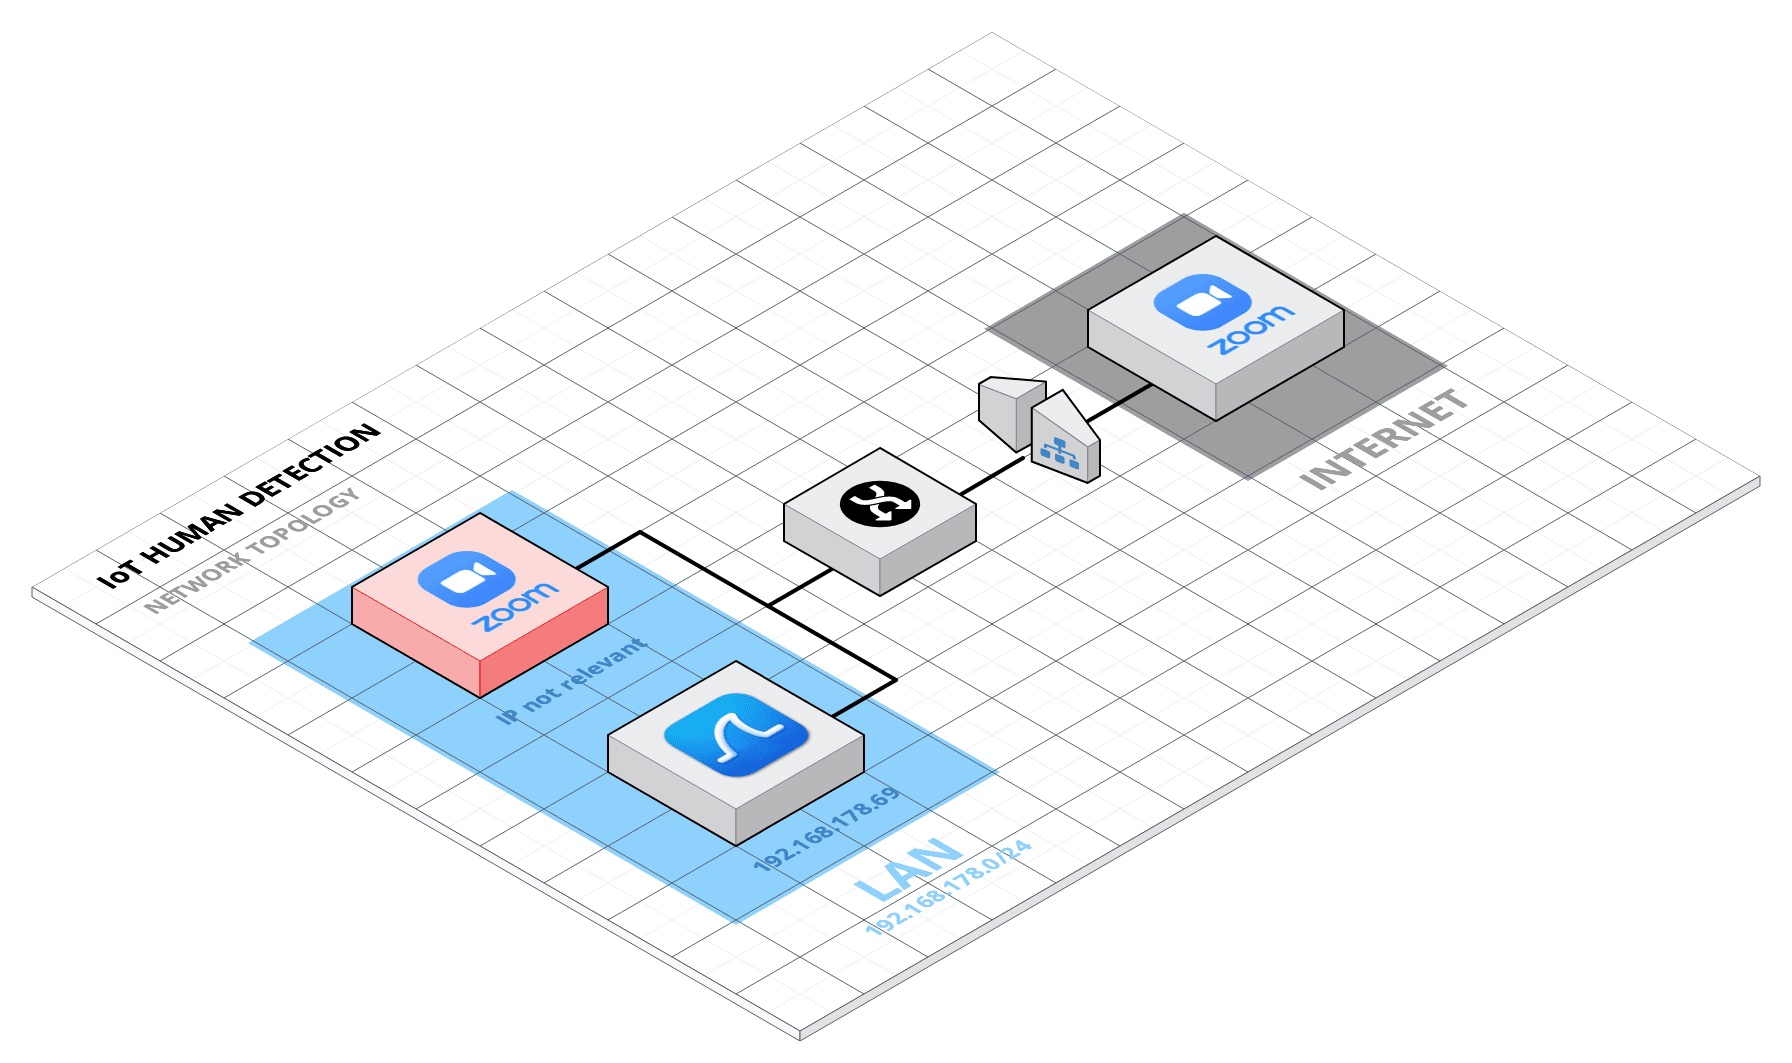
\includegraphics[width=10cm]{assets/Spy-Your-Mate-Topology.png}
	\caption{Network Topology: a simplified version of the LAN, target in red.}
	\label{fig::net-topology}
\end{figure}

\subsection[]{Traffic Generation}

Traffic generation was performed using the PC dumping the network traffic as a participant of a Zoom call, in which the target PC was the administrator and had the webcam turned on. The IP address of the eavesdropper was \texttt{192.168.178.69}. Since Zoom is not a \textit{Peer-To-Peer} application, an IP was needed in order to clean out the traffic from other unwanted destinations (sources). For this purpose an application firewall (\texttt{Little Snitch 5.4.1}) was used: it allowed to visualize a list of addresses used by Zoom to relay the traffic, see figure \ref{fig::little-snitch}. This allowed to get an idea of the range of IP addresses that the service provider used to perform the operation. \\ The time period in which someone was framed by the webcam was about 20 minutes, the same for the background only, for a total of 40 minutes.

\begin{figure}[h!]
	\centering
	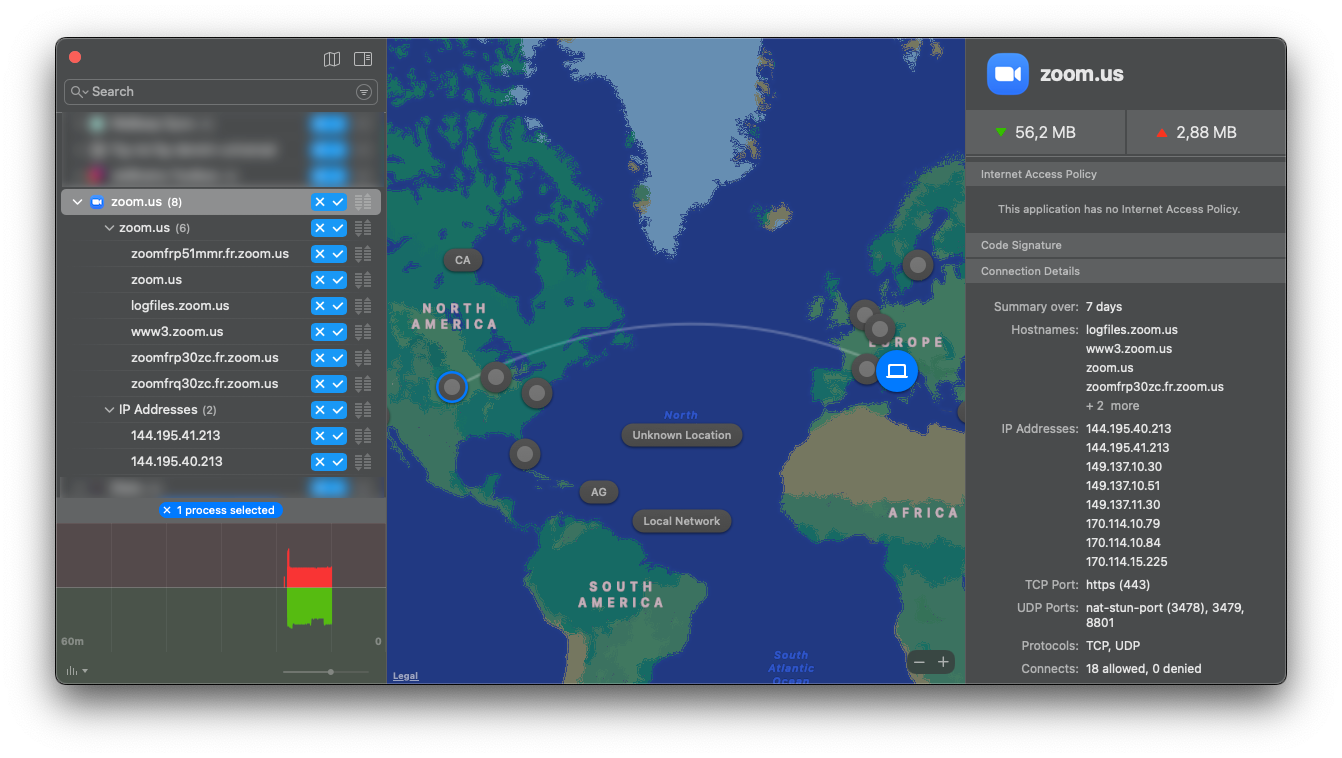
\includegraphics[width=15cm]{assets/little-snitch.png}
	\caption{Little Snitch instance, visualizing Zoom.US traffic (\textit{IP addresses don't correspond to the Juputer Notebook's ones because this screenshot was taken in a second moment})}
	\label{fig::little-snitch}
\end{figure}

\subsection{Traffic Acquisition}

Traffic acquisition was performed using \texttt{Wireshark} to acquire a \textit{Packet CAPture} (PCAP) file, from which some interesting information was extracted and exported in \textit{Comma Separated Value} (CSV) format, using \texttt{tshark}. The latter is presented in a terminal fashion, and the command used was:

\begin{commandline}
	\begin{verbatim}
		$ tshark -r "dataset-zoom-us-20+20_min.pcapng" -T fields -e 
		frame.time -e ip.src -e ip.dst -e ip.proto -e frame.len -E header=y 
		-E separator=, > "zoom_dataset.csv" -Y 'ip.addr == 149.137.12.48'
	\end{verbatim}
\end{commandline}
Said command allowed to export a CSV with the following characteristics (columns):

\begin{itemize}
	\item Timestamp;
	\item Source IP address;
	\item Destination IP address;
	\item Protocol;
	\item Frame Length.
\end{itemize}
From an initial network dump of \texttt{8.43 GB}, this allowed to narrow down to only \texttt{10.8 MB}.

%------------------------------------------------

\section{Node-RED Setup}

In order to acquire a \textit{Ground Truth}, and represent it, a \textit{Node-RED} dashboard was used. In the figures below it is possible to see the \textit{flow} used (Figure \ref{fig::node-red-flow}), and the dashboard itself (Figure \ref{fig::node-red-dashboard}). \\ Node-RED was running in a Docker container: so the CSV generated and (at the end) parsed were inputted using a remote shell connection.

\begin{figure}[h!]
	\centering
	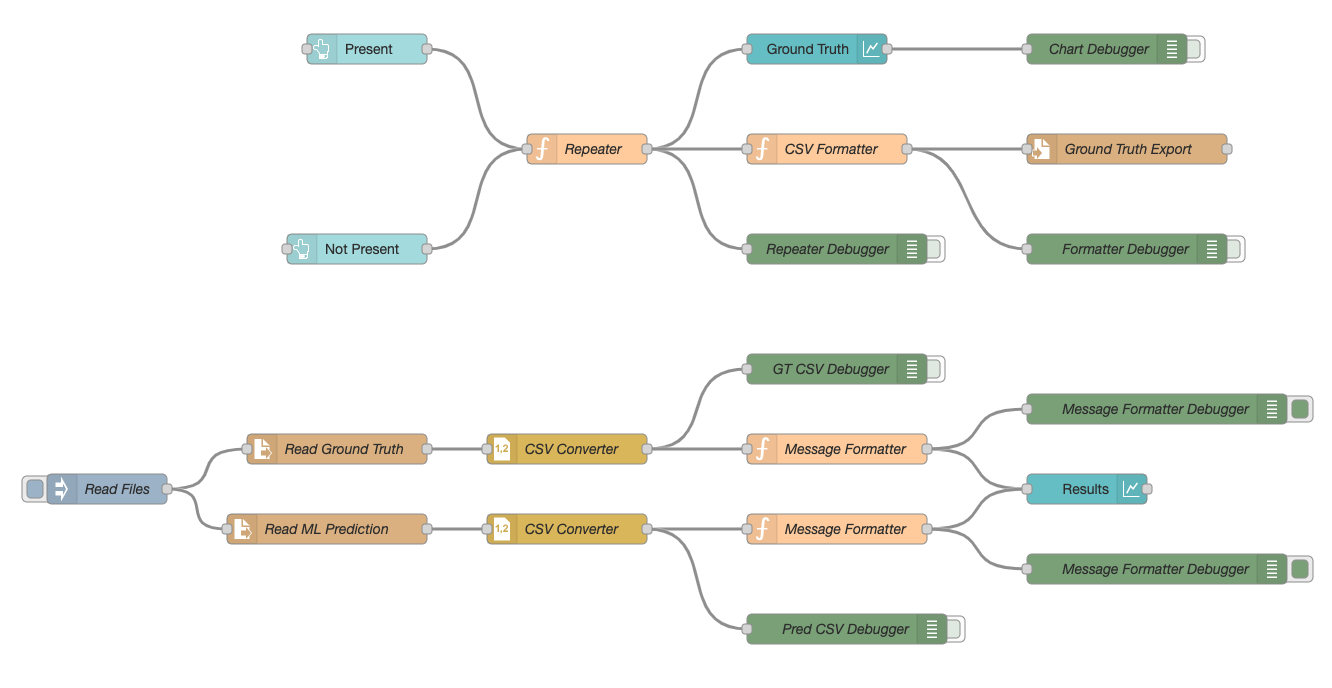
\includegraphics[width=12cm]{assets/node-red-flow.png}
	\caption{Node-RED Flow}
	\label{fig::node-red-flow}
\end{figure}
The ground truth consisted, as mentioned above, in a CSV reporting the \texttt{timestamp} and the value \texttt{1} if someone was framed, otherwise \texttt{0}.

\begin{figure}[h!]
	\centering
	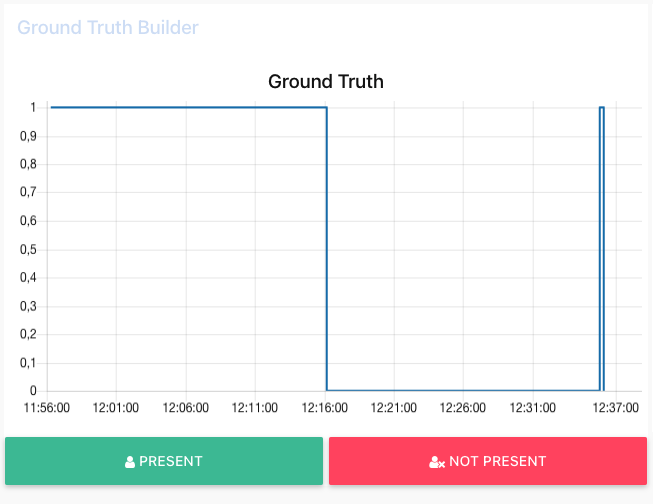
\includegraphics[width=8cm]{assets/ground-truth-builder.png}
	\caption{Node-RED Ground Truth Builder}
	\label{fig::node-red-dashboard}
\end{figure}

\section{Features and Data Visualization}

Everything disclosed in the previous section was used as an input for the Jupyter Notebook (which can be found in the repository mentioned in the introduction). The most technical details won't be addressed in this report, since every step is commented in the code itself. \\ On the other hand, in this section some remarks about the data acquired (before the model training) will be given. \\ The approach used to select the features was incremental: starting with few features, visualizing them graphically and trying to train the model. The features used were: \texttt{PacketNumber} (\textit{number of packets within a time interval of 450 ms}), \texttt{PacketIntervalAvg} (\textit{average amount of time between packets within 450 ms} - figure \ref{fig::avg-inter-time}), \texttt{PacketSizeAvg} (\textit{average packet size} - figure \ref{fig::avg-pkt-size}), \texttt{PacketSizeStd}, \texttt{PacketSizeMed}, \texttt{PacketSizeMin}, \texttt{PacketSizeMax}, \texttt{InboundCount} (\textit{number of packets received by the eavesdropper} - figure \ref{fig::inbound-traffic}), \texttt{OutboundCount} (\textit{number of packets sent by the eavesdropper}). \\ The correlation matrix between said features can be seen in figure \ref{fig::correlation-matrix}.

\begin{figure}[h!]
	\centering
	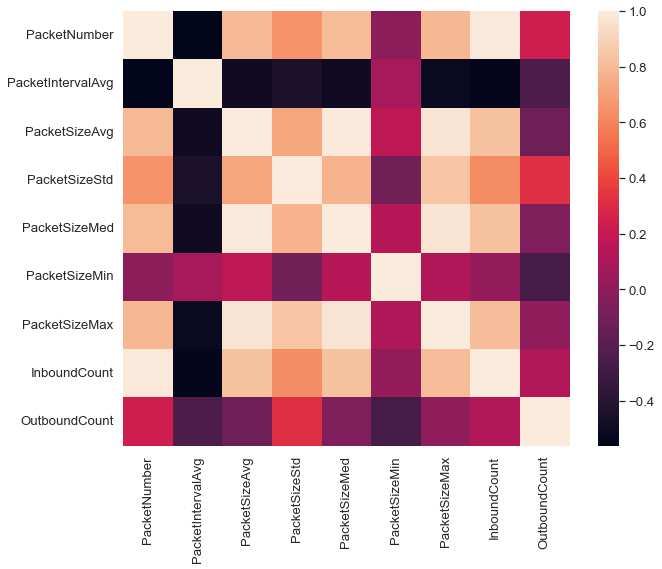
\includegraphics[width=10cm]{assets/correlation.png}
	\caption{Selected features correlation matrix}
	\label{fig::correlation-matrix}
\end{figure}
Plotting some of those features, with respect to the ground truth (pink line), it is evident when someone if framed and when not, despite the fact that some features are correlated (not completely) with some others.

\begin{figure}[h!]
	\centering
	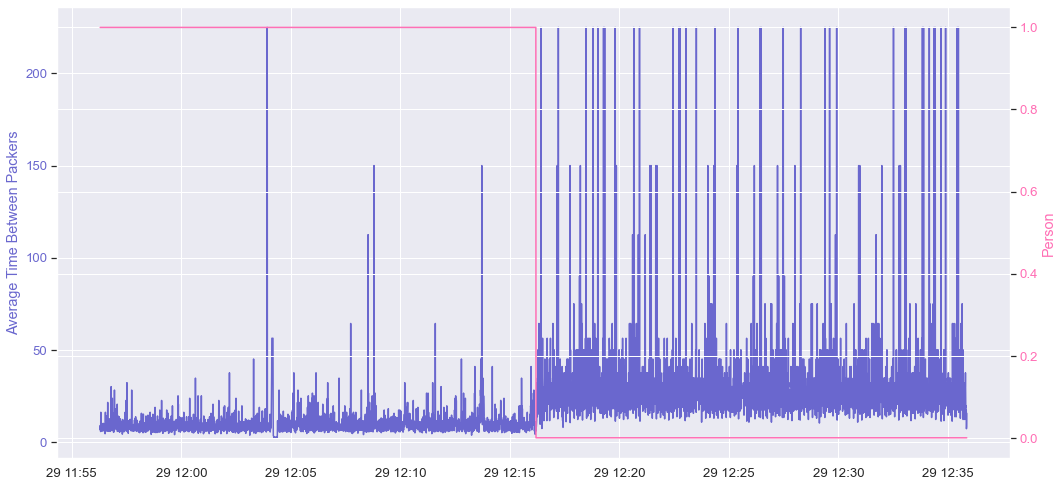
\includegraphics[width=12cm]{assets/avg-inter-time.png}
	\caption{Average Time Between Packets}
	\label{fig::avg-inter-time}
\end{figure}

\begin{figure}[h!]
	\centering
	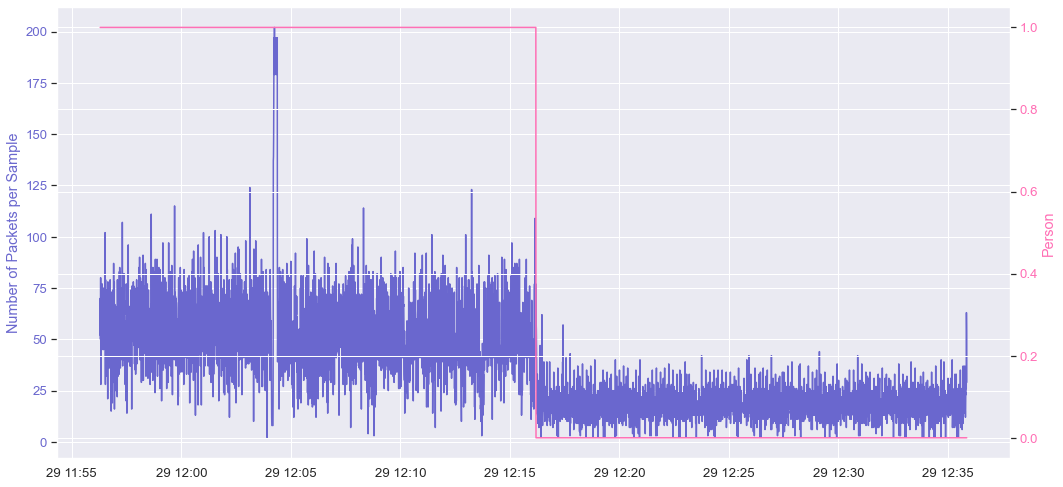
\includegraphics[width=12cm]{assets/packets-per-sample.png}
	\caption{Packets per Sample of 450 ms}
	\label{fig::pkt-per-sample}
\end{figure}

\begin{figure}[h!]
	\centering
	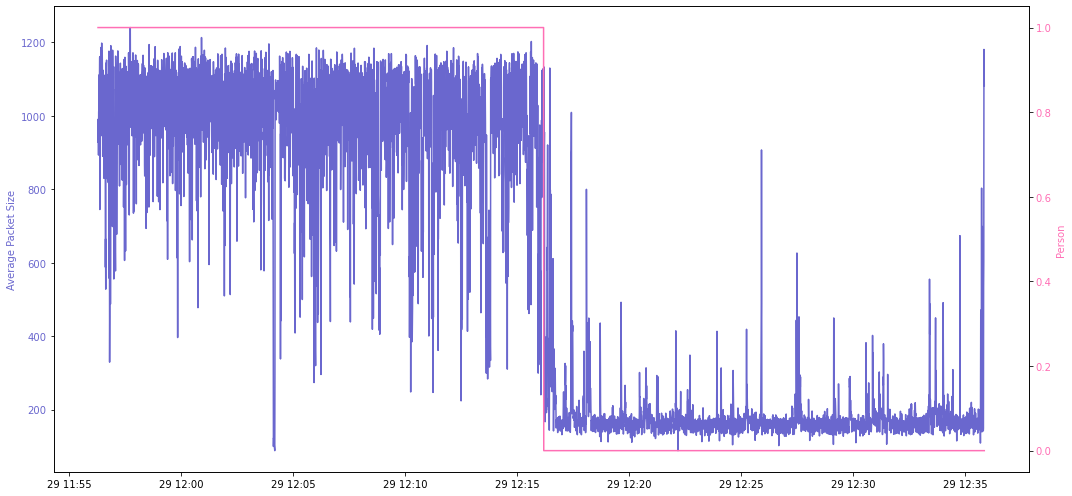
\includegraphics[width=12cm]{assets/avg-pkt-size.png}
	\caption{Average Packet Size within a Sample of 450 ms}
	\label{fig::avg-pkt-size}
\end{figure}

\begin{figure}[h!]
	\centering
	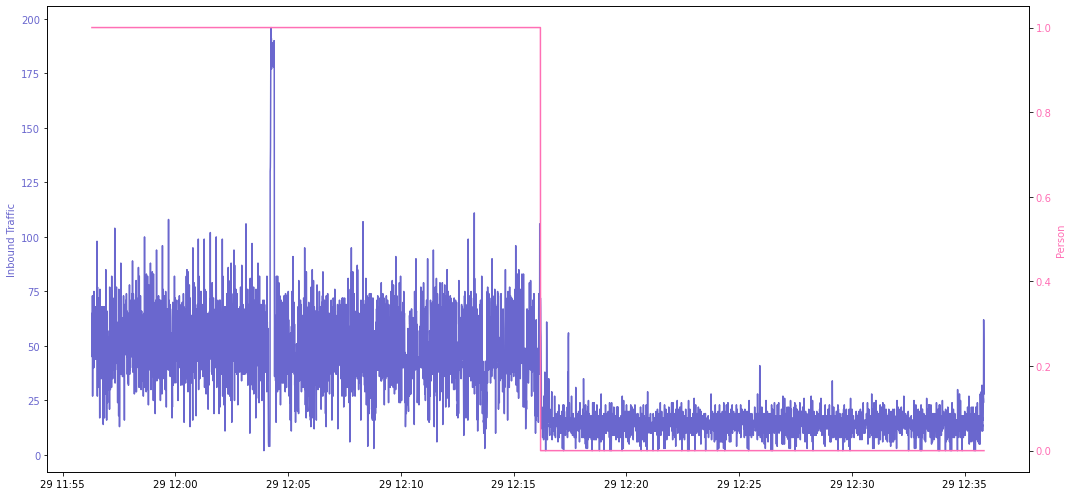
\includegraphics[width=12cm]{assets/inbound-traffic.png}
	\caption{Inbound Traffic}
	\label{fig::inbound-traffic}
\end{figure}

In the Jupyter Notebook are attached some other diagrams aimed at visualizing the data frame we are dealing with and also the selected features.

\newpage~\newpage
\section{Results}

As anticipated by the data visualization, the results were very accurate. The ML algorithms tested were: \textit{Random Forest}, \textit{K-Nearest Neighbor}, \textit{Support Vector Machine}, \textit{Logistic Regression}. \\
Every algorithm tested presented very similar results, with the lowest accuracy reported of around 97\%, and the highest one of 99\%. Everything is reported in the Jupyter Notebook, however in this section will be included some more information about only 2 of the trained models since they all behaved the same.

\subsection[]{Random Forest}

\begin{table}[h!]
	\centering
	\begin{tabular}{l|llll}
		\toprule 
		Label & Precision (\%) & Recall (\%) & F1 Score (\%) \\
		\midrule
		\rowcolor{black!10} \texttt{Background (0)} & 99.6047 & 97.2973 & 98.4375 \\
		\texttt{Person (1)} & 97.4122 & 99.6219 & 98.5047 \\
		\bottomrule
	\end{tabular}
	\caption{\textit{Random Forest} trained model metrics}
	\label{tab:rf-results}
 \end{table}

\begin{figure}[h!]
	\centering
	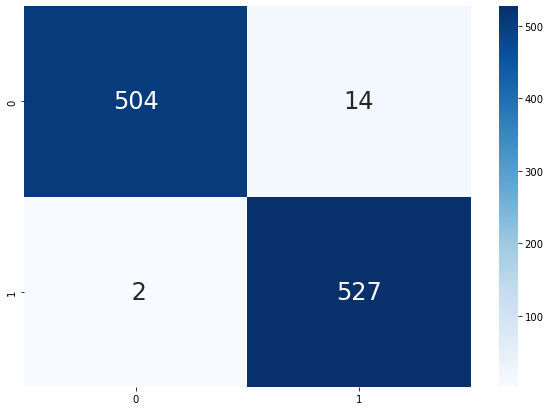
\includegraphics[width=6cm]{assets/rf-confusion-matrix.png}
	\caption{Random Forest Model Confusion Matrix}
	\label{fig::rf-confusion-matrix}
\end{figure}

\subsection[]{Support Vector Machine}

\begin{table}[h!]
	\centering
	\begin{tabular}{l|llll}
		\toprule 
		Label & Precision (\%) & Recall (\%) & F1 Score (\%) \\
		\midrule
		\rowcolor{black!10} \texttt{Background (0)} & 97.5285 & 99.0347 & 98.2759 \\
		\texttt{Person (1)} & 99.0403 & 97.5425 & 98.2857 \\
		\bottomrule
	\end{tabular}
	\caption{\textit{Support Vector Machine} trained model metrics}
	\label{tab:svm-results}
 \end{table}

\begin{figure}[h!]
	\centering
	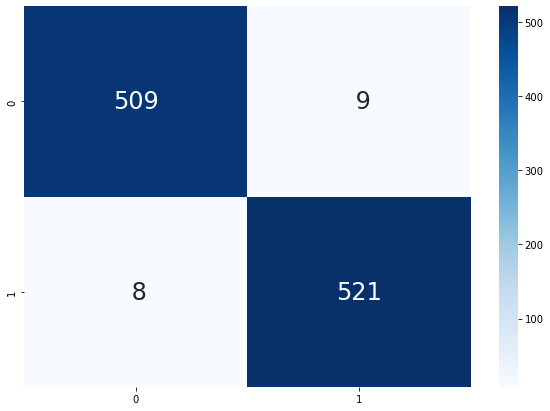
\includegraphics[width=6cm]{assets/SVM-confusion-matrix.png}
	\caption{Support Vector Machine Model Confusion Matrix}
	\label{fig::svm-confusion-matrix}
\end{figure}

\subsection[]{Predicted vs Actual Data Visualization}

Taking as an example the RF model, the actual predicted vs actual values chart looks something like figure \ref{fig::rf-predicted-vs-actual-total}, and the SVM one, like figure \ref{fig::svm-predicted-vs-actual-total}: this is completely unreadable from this report. In the Jupyter Notebook the plot can be enlarged and inspected, the values match almost completely; this can be noticed in figure \ref{fig::rf-predicted-vs-actual-enlarged}, an enlargement of figure \ref{fig::rf-predicted-vs-actual-total}, with some line tweaking to make the visualization easier.

\begin{figure}[h!]
	\centering
	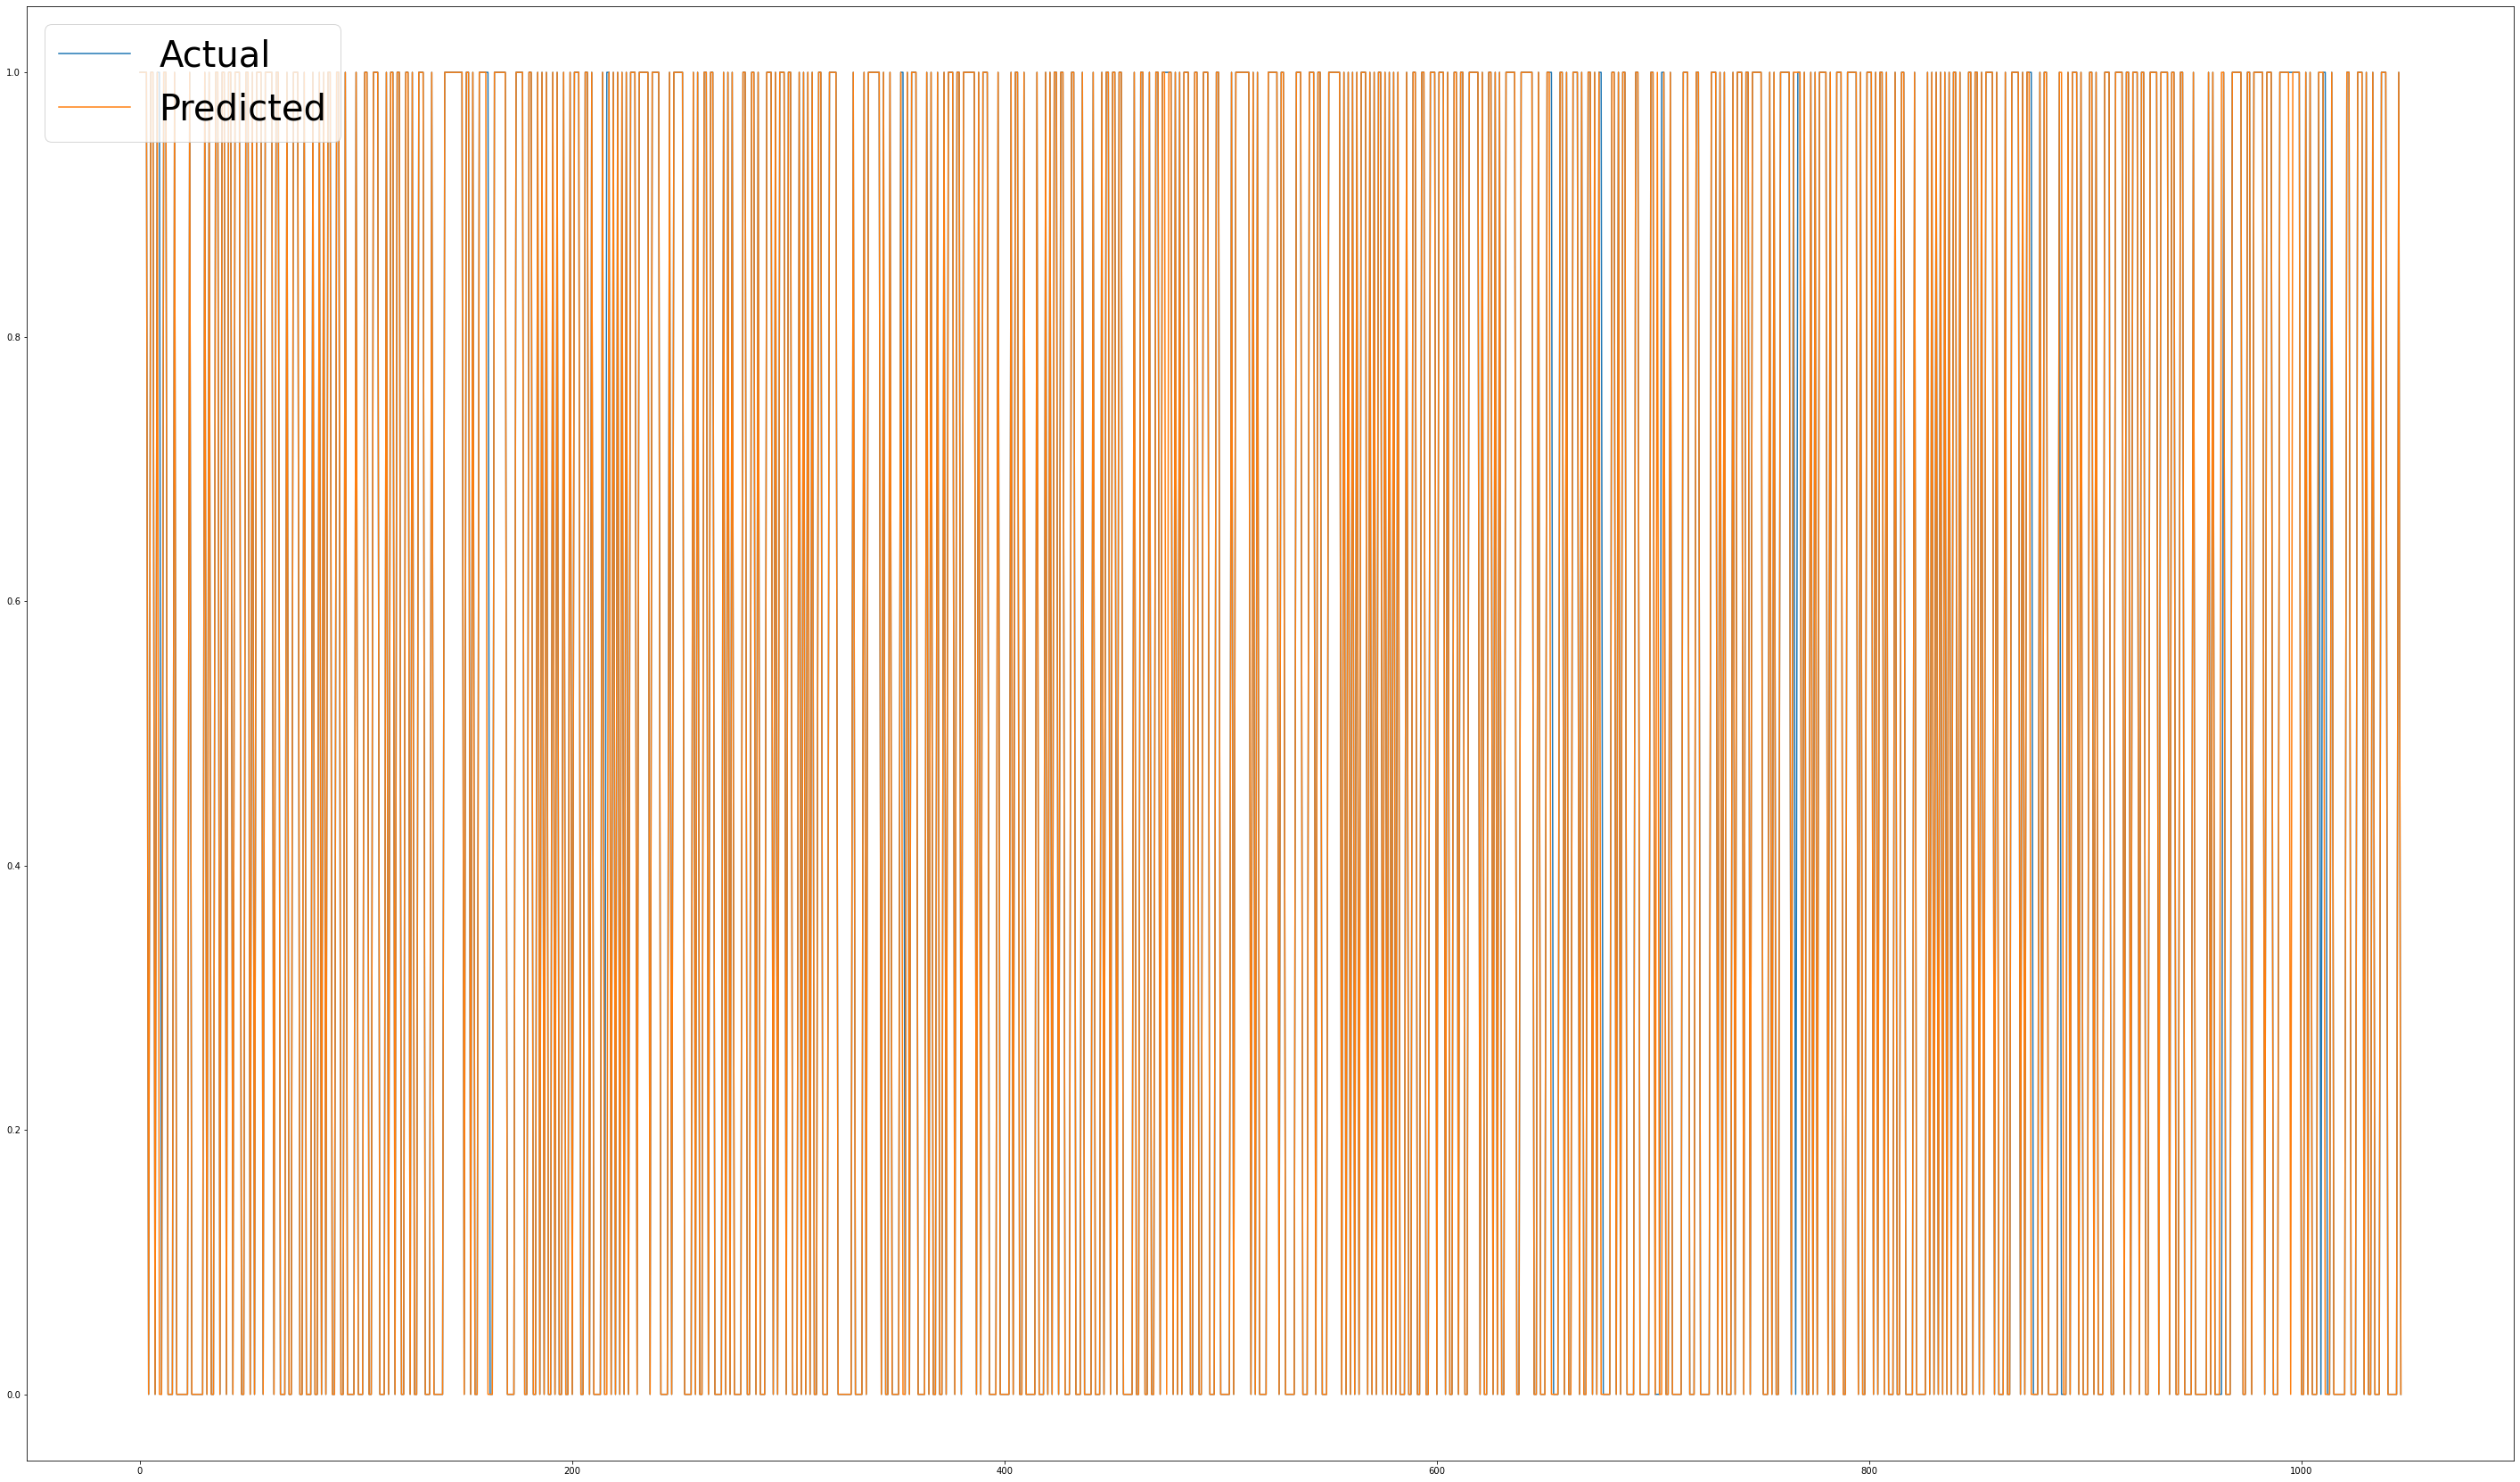
\includegraphics[width=9.5cm]{assets/svm-diagram-predicted-vs-actual-total.png}
	\caption{Random Forest Model Predicted (orange) vs Actual (blue) Values}
	\label{fig::rf-predicted-vs-actual-total}
\end{figure}

\begin{figure}[h!]
	\centering
	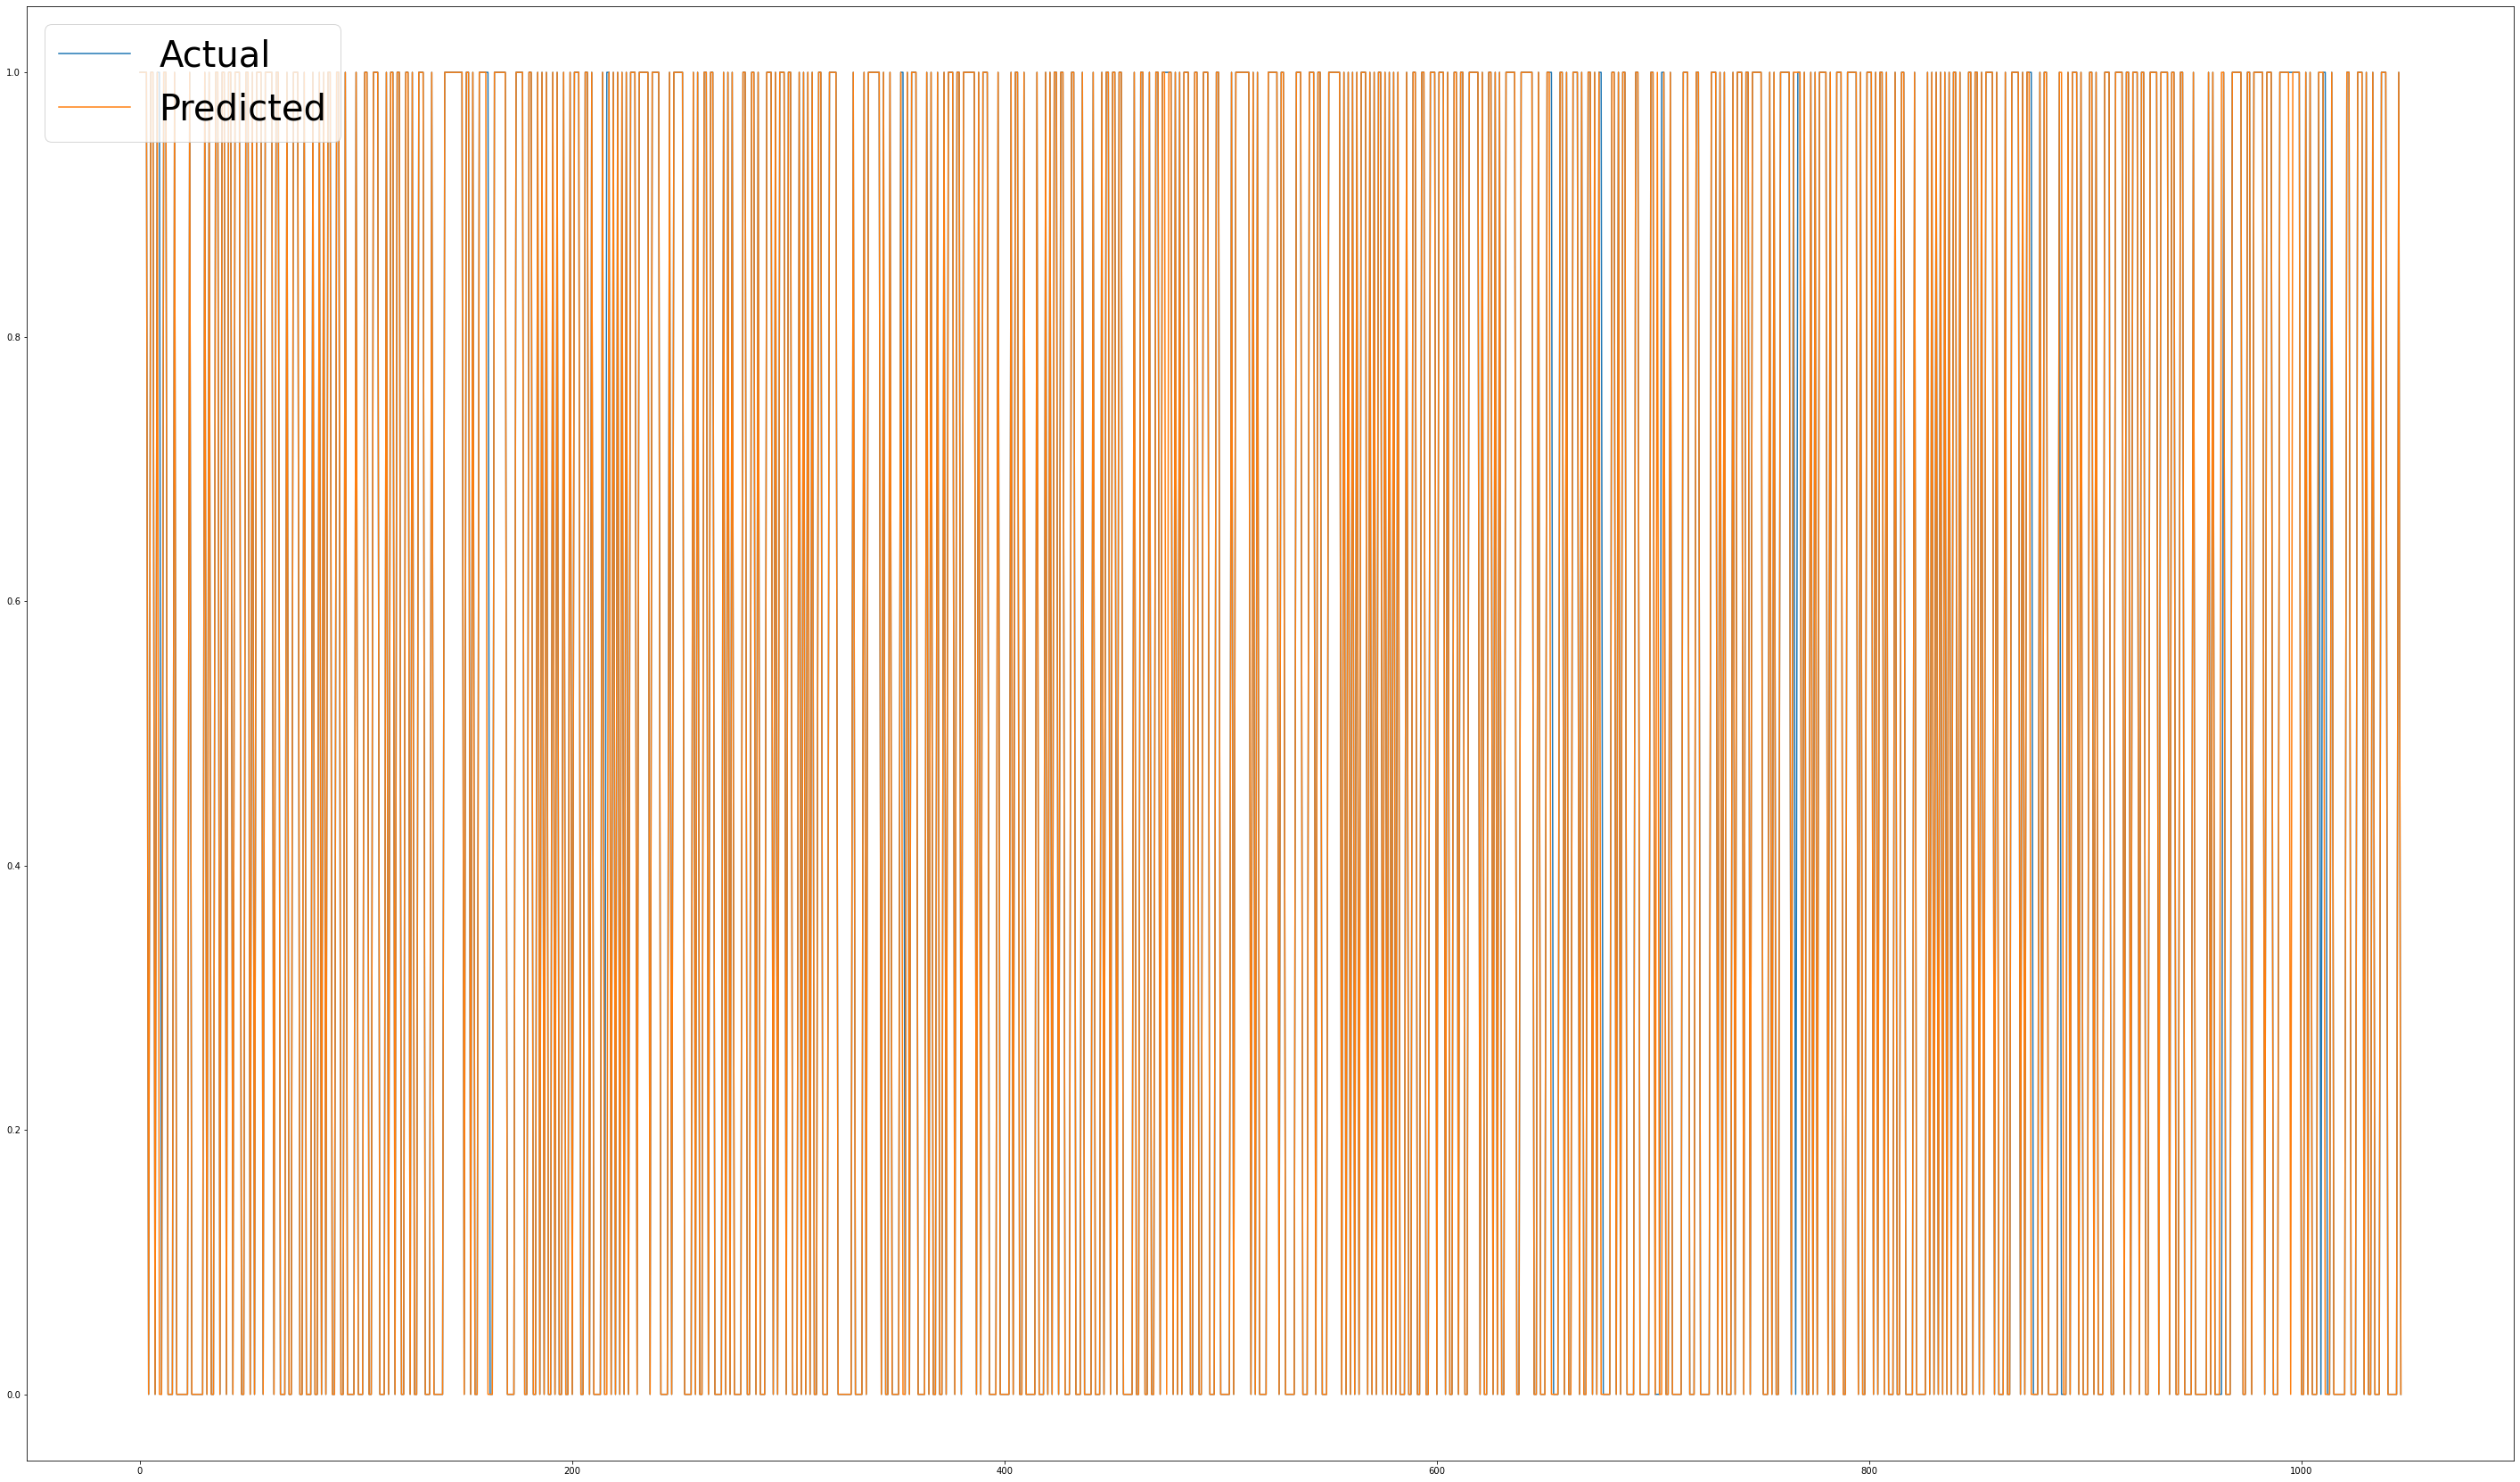
\includegraphics[width=9.5cm]{assets/svm-diagram-predicted-vs-actual-total.png}
	\caption{Support Vector Machine Model Predicted (orange) vs Actual (blue) Values}
	\label{fig::svm-predicted-vs-actual-total}
\end{figure}

\begin{figure}[h!]
	\centering
	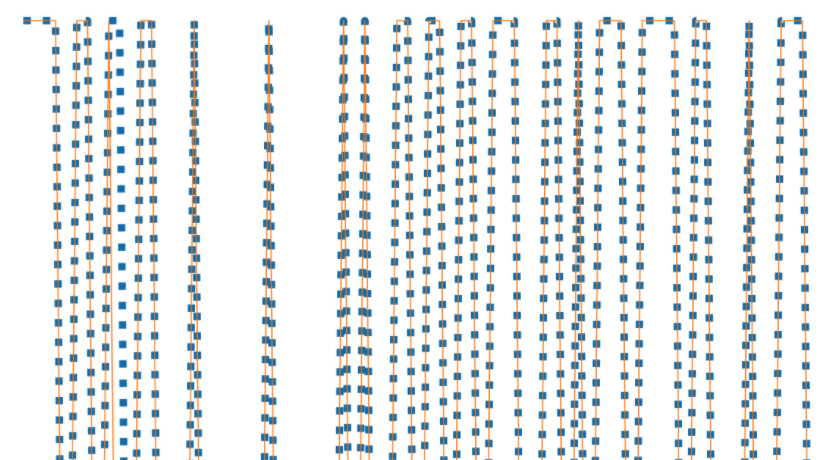
\includegraphics[width=9cm]{assets/rf-predicted-vs-actual-enlarged.png}
	\caption{Random Forest Model Predicted (orange) vs Actual (blue) Values - Enlarged (\textit{as expected from a 99\% accuracy, the lines overlap almost every time}).}
	\label{fig::rf-predicted-vs-actual-enlarged}
\end{figure}

\subsection[]{Node-RED Results Chart}

Results were exported from the Jupyter Notebook in CSV format, then copy-pasted in the Node-RED's docker container, in order to be visualized using the dedicated dashboard. Since the procedure would have been the same for every algorithm, and so the results, only the RF model ones were plotted using this application.
 
%----------------------------------------------------------------------------------------

\end{document}
